\documentclass{article}

% For adjusting images
\usepackage{adjustbox}
% For functions like \binom
\usepackage{amsmath}
% For functions like \wedge \subseteq \mathbb
\usepackage{amssymb}
% 312 Font
\usepackage{charter}
% Circuit diagrams
\usepackage{circuitikz}
% Custom lists
\usepackage{enumitem}
% Page margins & pagestyles
\usepackage{fullpage}
% Font encoding
\usepackage[T1]{fontenc}
% Colored boxes around the 'solution' environment
\usepackage{mdframed}
% Used for making Karnaugh Maps
\usepackage{tikz}
\usetikzlibrary{matrix,calc}
% For color
\usepackage[dvipsnames]{xcolor}

% Defines a solution environment that creates a green box around text inside.
\mdfdefinestyle{SolutionFrame}{linecolor=green!60!black,linewidth=1pt}
\newenvironment{solution}{\begin{mdframed}[style=SolutionFrame]}{\end{mdframed}}

% Enumerate with (a),(b),(c),...
\newenvironment{enum}{\begin{enumerate}[label={(\alph*)}]}{\end{enumerate}}

% Put a dot after section titles
\renewcommand\thesection{\arabic{section}.}
\renewcommand\thesubsection{\arabic{section}.\arabic{subsection}}

% Hide the Date
\date{}
% Hide page numbers
\pagenumbering{gobble}

\begin{document}
    % Used for making Karnaugh Maps
    % \documentclass{standalone}

% \usepackage{tikz}
% \usetikzlibrary{matrix,calc}

\newcommand{\p}{\phantom{0}}
\newcommand{\pp}{\phantom{00}}

% Isolated term
%#1 - Optional. Space between node and grouping line. Default=0
%#2 - Node
%#3 - Fill color
\newcommand{\isolated}[3][0] {
    \draw [rounded corners=3pt, fill=#3, opacity=0.3]
    ($(#2.north west)+(135:#1)$) rectangle ($(#2.south east)+(-45:#1)$);
}

% Internal group
%#1 - Optional. Space between node and grouping line. Default=0
%#2 - Top left node
%#3 - Bottom right node
%#4 - Fill color
\newcommand{\internal}[4][0] {
    \draw [rounded corners=3pt, fill=#4, opacity=0.3]
    ($(#2.north west)+(135:#1)$) rectangle ($(#3.south east)+(-45:#1)$);
}

% Horizontal border group
%#1 - Optional. Space between node and grouping line. Default=0
%#2 - Top left node
%#3 - Bottom right node
%#4 - Fill color
\newcommand{\horizontal}[4][0] {
    \draw [rounded corners=3pt, fill=#4, opacity=0.3]
    ($(rf.east |- #2.north)+(90:#1)$) -| ($(#2.east)+(0:#1)$) |- ($(rf.east |- #3.south)+(-90:#1)$)
    ($(cf.west |- #2.north)+(90:#1)$) -| ($(#3.west)+(180:#1)$) |- ($(cf.west |- #3.south)+(-90:#1)$);
}

% Vertical border group
%#1 - Optional. Space between node and grouping line. Default=0
%#2 - Top left node
%#3 - Bottom right node
%#4 - Fill color
\newcommand{\vertical}[4][0] {
    \draw [rounded corners=3pt, fill=#4, opacity=0.3]
    ($(cf.south -| #2.west)+(180:#1)$) |- ($(#2.south)+(-90:#1)$) -| ($(cf.south -| #3.east)+(0:#1)$)
    ($(rf.north -| #2.west)+(180:#1)$) |- ($(#3.north)+(90:#1)$) -| ($(rf.north -| #3.east)+(0:#1)$);
}

% Corners group (Only used in 4x4s)
%#1 - Optional. Space between node and grouping line. Default=0
%#2 - Fill color
\newcommand{\corners}[2][0] {
    \draw [rounded corners=3pt, opacity=.3]
    ($(rf.east |- 0000.south)+(-90:#1)$) -| ($(0000.east |- cf.south)+(0:#1)$)
    ($(rf.east |- 0010.north)+(90:#1)$) -| ($(0010.east |- rf.north)+(0:#1)$)
    ($(cf.west |- 1000.south)+(-90:#1)$) -| ($(1000.west |- cf.south)+(180:#1)$)
    ($(cf.west |- 1010.north)+(90:#1)$) -| ($(1010.west |- rf.north)+(180:#1)$);
    
    \fill [rounded corners=3pt, fill=#2, opacity=.3]
    ($(rf.east |- 0000.south)+(-90:#1)$) -|  ($(0000.east |- cf.south)+(0:#1)$) [sharp corners] ($(rf.east |- 0000.south)+(-90:#1)$) |-  ($(0000.east |- cf.south)+(0:#1)$)
    
    ($(rf.east |- 0010.north)+(90:#1)$) -| ($(0010.east |- rf.north)+(0:#1)$) [sharp corners] ($(rf.east |- 0010.north)+(90:#1)$) |- ($(0010.east |- rf.north)+(0:#1)$)
    
    ($(cf.west |- 1000.south)+(-90:#1)$) -| ($(1000.west |- cf.south)+(180:#1)$) [sharp corners]($(cf.west |- 1000.south)+(-90:#1)$) |- ($(1000.west |- cf.south)+(180:#1)$)
    
    ($(cf.west |- 1010.north)+(90:#1)$) -| ($(1010.west |- rf.north)+(180:#1)$) [sharp corners] ($(cf.west |- 1010.north)+(90:#1)$) |- ($(1010.west |- rf.north)+(180:#1)$);
}

% Empty Karnaugh map 4x4
\newenvironment{Karnaugh4}[4] {
    \begin{tikzpicture}[baseline=(current bounding box.north),scale=0.8]
        \draw (0,0) grid (4,4);
        \draw (0,4) -- node [pos=0.7,above right,anchor=south west] {#1#2}
            node [pos=0.7,below left,anchor=north east] {#3#4} ++(135:1);
        \matrix (mapa) [
            matrix of nodes,
            column sep={0.8cm,between origins},
            row sep={0.8cm,between origins},
            every node/.style={minimum size=0.3mm},
            anchor=0010.center,
            ampersand replacement=\&
        ] at (0.5,0.5) {
                       \& |(c00)|  00 \& |(c01)|  01 \& |(c11)|  11 \& |(c10)|  10 \& |(cf)| \pp \\
            |(r00)| 00 \& |(0000)| \p \& |(0100)| \p \& |(1100)| \p \& |(1000)| \p \& \\
            |(r01)| 01 \& |(0001)| \p \& |(0101)| \p \& |(1101)| \p \& |(1001)| \p \& \\
            |(r11)| 11 \& |(0011)| \p \& |(0111)| \p \& |(1111)| \p \& |(1011)| \p \& \\
            |(r10)| 10 \& |(0010)| \p \& |(0110)| \p \& |(1110)| \p \& |(1010)| \p \& \\
            |(rf)| \pp \& \& \& \& \& \\
        };
}
{\end{tikzpicture}}

% Empty Karnaugh map 2x4
\newenvironment{Karnaugh3}[3] {
    \begin{tikzpicture}[baseline=(current bounding box.north),scale=0.8]
        \draw (0,0) grid (4,2);
        \draw (0,2) -- node [pos=0.7,above right,anchor=south west] {#1#2}
            node [pos=0.7,below left,anchor=north east] {#3} ++(135:1);
        \matrix (mapa) [
            matrix of nodes,
            column sep={0.8cm,between origins},
            row sep={0.8cm,between origins},
            every node/.style={minimum size=0.3mm},
            anchor=001.center,
            ampersand replacement=\&
        ] at (0.5,0.5) {
                      \& |(c00)| 00 \& |(c01)| 01 \& |(c11)| 11 \& |(c10)| 10 \& |(cf)| \pp \\
            |(r00)| 0 \& |(000)| \p \& |(010)| \p \& |(110)| \p \& |(100)| \p \& \\
            |(r01)| 1 \& |(001)| \p \& |(011)| \p \& |(111)| \p \& |(101)| \p \& \\
            |(rf)| \pp \& \& \& \& \& \\
        };
}
{\end{tikzpicture}}

% Empty Karnaugh map 2x2
\newenvironment{Karnaugh2}[2] {
    \begin{tikzpicture}[baseline=(current bounding box.north),scale=0.8]
        \draw (0,0) grid (2,2);
        \draw (0,2) -- node [pos=0.7,above right,anchor=south west] {#1}
            node [pos=0.7,below left,anchor=north east] {#2} ++(135:1);
        \matrix (mapa) [
            matrix of nodes,
            column sep={0.8cm,between origins},
            row sep={0.8cm,between origins},
            every node/.style={minimum size=0.3mm},
            anchor=01.center,
            ampersand replacement=\&
        ] at (0.5,0.5) {
                      \& |(c00)| 0 \& |(c01)| 1 \\
            |(r00)| 0 \& |(00)| \p \& |(10)| \p \\
            |(r01)| 1 \& |(01)| \p \& |(11)| \p \\
        };
}
{\end{tikzpicture}}

% Places 1s in listed positions
\newcommand{\ones}[1] {
    \foreach \x in {#1}
        \path (\x) node {1};
}

% Places 0s in listed positions
\newcommand{\zeroes}[1] {
    \foreach \x in {#1}
        \path (\x) node {0};
}

% Places Xs in listed positions
\newcommand{\exes}[1] {
    \foreach \x in {#1}
        \path (\x) node {X};
}

% Examples (Uncomment document type & packages at the top of the file too)

% \begin{document}
%     \begin{Karnaugh4}{a}{b}{c}{d}
%         \zeroes{0000,0001,0010,0011,0100,0101,0110,0111,
%             1000,1001,1010,1011,1100,1101,1110,1111}
%         \internal{0000}{1000}{red}
%         \internal{0101}{1111}{purple}
%         \vertical[3pt]{1100}{1010}{blue}
%         \corners[2pt]{orange}
%         \horizontal{0001}{1011}{green}
%     \end{Karnaugh4}
    
%     \begin{Karnaugh3}{X}{Y}{Z}
%         \ones{110,001}
%         \zeroes{000,010,111,101}
%         \exes{100,011}
%         \internal{110}{100}{green}
%         \internal{001}{011}{}
%     \end{Karnaugh3}

%     \begin{Karnaugh2}{I}{J}
%         \ones{10,01}
%         \zeroes{00,11}
%         \isolated{10}{green}
%         \isolated{01}{red}
%     \end{Karnaugh2}
% \end{document}

    \begin{titlepage}
        \centering
        \null
        \vspace{5cm}
        {\Huge CSE 369 Lab 3\par}
        \vspace{0.5cm}
        {\Large Digital Design using FPGAs \par}
        \vfill
        {\hfill \Large Isaac Wu \par}
        {\hfill \large 2360957 \par}
        {\hfill \large \today \par}
    \end{titlepage}

\section{Karnaugh Maps}
    \begin{enum}
        \item Discounted
            \begin{solution}
                \begin{center}
                    \begin{tabular}{c|c|c|c||c}
                        U & P & C & Mark & Discounted \\ \hline
                        0 & 0 & 0 & 0 & 0 \\ \hline
                        0 & 0 & 0 & 1 & 0 \\ \hline
                        0 & 0 & 1 & 0 & 0 \\ \hline
                        0 & 0 & 1 & 1 & 0 \\ \hline
                        0 & 1 & 0 & 0 & X \\ \hline
                        0 & 1 & 0 & 1 & X \\ \hline
                        0 & 1 & 1 & 0 & 1 \\ \hline
                        0 & 1 & 1 & 1 & 1 \\ \hline
                        1 & 0 & 0 & 0 & 0 \\ \hline
                        1 & 0 & 0 & 1 & 0 \\ \hline
                        1 & 0 & 1 & 0 & 1 \\ \hline
                        1 & 0 & 1 & 1 & 1 \\ \hline
                        1 & 1 & 0 & 0 & 1 \\ \hline
                        1 & 1 & 0 & 1 & 1 \\ \hline
                        1 & 1 & 1 & 0 & X \\ \hline
                        1 & 1 & 1 & 1 & X \\ \hline
                    \end{tabular}
                    \vfill
                    
                    \begin{Karnaugh4}{U}{P}{C}{M}
                        \ones{0110,0111,1010,1011,1100,1101}
                        \zeroes{0000,0001,0010,0011,1000,1001}
                        \exes{0100,0101,1110,1111}

                        \internal{0100}{1110}{blue}
                        \internal{1111}{1010}{green}
                    \end{Karnaugh4}
                    $$\text{Discounted}=\textcolor{blue}{\mathbf{P}}+\textcolor{ForestGreen}{\mathbf{UC}}$$
                \end{center}
            \end{solution}

        \newpage
        \item Stolen
            \begin{solution}
                \begin{center}
                    \begin{tabular}{c|c|c|c||c}
                        U & P & C & Mark & Stolen \\ \hline
                        0 & 0 & 0 & 0 & 1 \\ \hline
                        0 & 0 & 0 & 1 & 0 \\ \hline
                        0 & 0 & 1 & 0 & 0 \\ \hline
                        0 & 0 & 1 & 1 & X \\ \hline
                        0 & 1 & 0 & 0 & X \\ \hline
                        0 & 1 & 0 & 1 & X \\ \hline
                        0 & 1 & 1 & 0 & 0 \\ \hline
                        0 & 1 & 1 & 1 & X \\ \hline
                        1 & 0 & 0 & 0 & 1 \\ \hline
                        1 & 0 & 0 & 1 & 0 \\ \hline
                        1 & 0 & 1 & 0 & 1 \\ \hline
                        1 & 0 & 1 & 1 & 0 \\ \hline
                        1 & 1 & 0 & 0 & 0 \\ \hline
                        1 & 1 & 0 & 1 & X \\ \hline
                        1 & 1 & 1 & 0 & X \\ \hline
                        1 & 1 & 1 & 1 & X \\ \hline
                    \end{tabular}
                    \vfill
                    
                    \begin{Karnaugh4}{U}{P}{C}{M}
                        \ones{0000,1000,1010}
                        \zeroes{0001,0010,0110,1001,1011,1100}
                        \exes{0011,0100,0101,0111,1101,1110,1111}

                        \internal{0000}{0100}{blue}
                        \vertical{1000}{1010}{green}
                    \end{Karnaugh4}
                    $$\text{Stolen}=\textcolor{blue}{\mathbf{\overline{U}\,\overline{C}\,\overline{M}}}+\textcolor{ForestGreen}{\mathbf{U\,\overline{P}\,\overline{M}}}$$
                \end{center}
            \end{solution}
    \end{enum}

\newpage
\section{Circuit Diagrams}
    \begin{enum}
        \item Discounted
            \begin{solution}
                \begin{center}
                    \begin{circuitikz}  \draw
                        (0,3) node (u) {U}
                        (0,2) node (p) {P}
                        (0,1) node (c) {C}
                        (0,0) node (m) {Mark}
                        (5,0) node (eq) {\boxed{P+UC}}
                        (6.5,2.28) node (out) {Discounted}

                        (3,2.75) node[and port] (and) {\hspace{-0.4em} AND}
                        (5,2.28) node[or port] (or) {OR}

                        (u) -- (and.in 1)
                        (c) -| (and.in 2)
                        
                        (and.out) |- (or.in 1)
                        (p) to[xing] ++(3.22,0) -- (or.in 2)
                        
                        (or.out) -- (out)
                        ;
                    \end{circuitikz}
                \end{center}
            \end{solution}

        \item Stolen
            \begin{solution}
                \begin{center}
                    \begin{circuitikz}  \draw
                        (0,4) node (u) {U}
                        (1.5,4) node[not port, scale=0.6] (not_u) {\hspace{-0.4em}\footnotesize NOT}
                        (0,2) node (p) {P}
                        (0,1) node (c) {C}
                        (0,0) node (m) {Mark}
                        (6.5,0) node (eq) {\boxed{\overline{U}\,\overline{C}\,\overline{M}+U\,\overline{P}\,\overline{M}\rightarrow\overline{(U+C+M)(\overline{U}+P+M)}}}
                        (6.5,2) node (out) {Stolen}

                        (4,3) node[or port, number inputs=3] (or_ucm) {OR}
                        (4,1) node[or port, number inputs=3] (or_upm) {OR}
                        (5.6,2) node[nand port] (nand) {\hspace{-0.4em}\footnotesize NAND}

                        (u) -- ++(.5,0) node[circle, draw, fill, scale=.25] (dot) {} -- (not_u)

                        (u) -- ++(0.5,0) |- (2.4,3.38) to[xing] (or_ucm.in 1)
                        (c) -- ++(0.75,0) -- ++(0,.75) to[xing] ++(0,.5) |- (2.4,3) to[xing] (or_ucm.in 2)
                        (m) -- ++(1,0) -- ++(0,1.75) to[xing] ++ (0,.5) |- (2.4,2.62) to[xing] (or_ucm.in 3)
                        (not_u.out) -- ++(.59,0) |- (or_upm.in 1)
                        (p) -- ++(2,0) |- (or_upm.in 2)
                        (m) -- ++(1,0) node[circle, draw, fill, scale=.25] (dot) {} -- ++(1.5,0) |- (or_upm.in 3)

                        (or_ucm.out) |- (nand.in 1)
                        (or_upm.out) |- (nand.in 2)

                        (nand.out) -- (out)
                        ;
                    \end{circuitikz}
                \end{center}
            \end{solution}
    \end{enum}

% \newpage
\clearpage
\section{ModelSim Simulation}
    \begin{solution}
        Here is the code for my recognizer circuit. I defined logic variables for U, P, C, and Mark to make it easier to translate the inputs. Then, using the logic calculated using the Karnaugh Maps above, I assigned values to Discounted and Stolen, two logic variables defined above. Then, I assigned the values of Discounted and Stolen to two LEDs to display the output of the calculation. \\
        \begin{minipage}[t]{0.9\linewidth}
            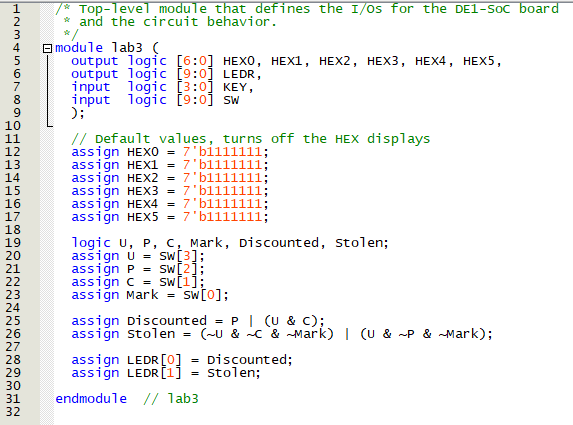
\includegraphics[width=0.9\linewidth]{Lab3/code.png}
        \end{minipage} \\
        This is the code for my test benchmark used to ensure correct functionality from my circuit. This code will run my lab3 module with all 16 combinations of switch inputs. \\
        \begin{minipage}[t]{0.9\linewidth}
            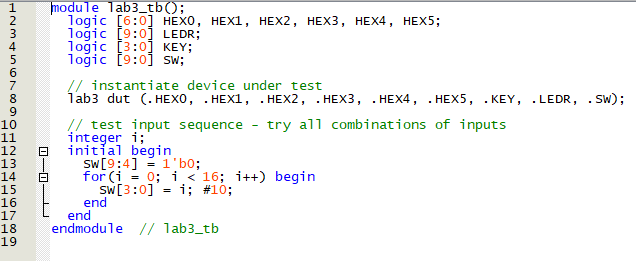
\includegraphics[width=0.9\linewidth]{Lab3/test_bench.png}
        \end{minipage}
        \newpage
        This is what my wave diagram looks like. The top 4 waves show the 4 switches alternating to test all 16 combinations. The bottom two waves are the LED output, with LEDR[0] corresponding to if a product is Discounted, and LEDR[1] if a product was stolen. \\
        \begin{minipage}[t]{0.9\linewidth}
            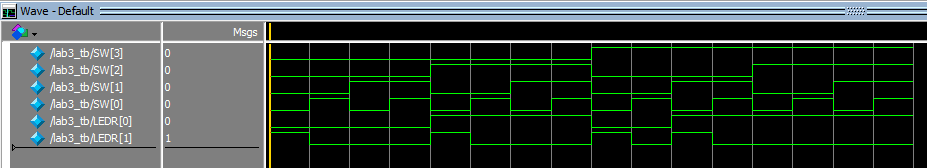
\includegraphics[width=0.9\linewidth]{Lab3/waves.png}
        \end{minipage}
    \end{solution}

\section{Misc.}
    How many hours (estimated) it took to complete this lab in total, including reading, planning, designing, coding, debugging, and testing.
    \begin{solution}
        It took around 7 hours to complete this lab.
    \end{solution}

\end{document}